\section{Results}
\label{sec:results}

\begin{figure}
  \centering
  \subfloat[Increments\label{fig:incnew}]{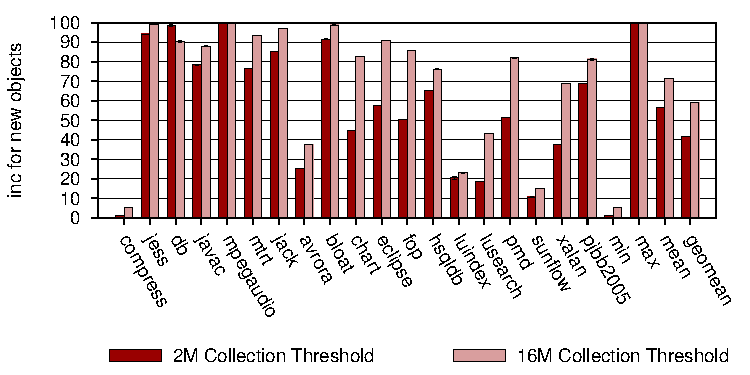
\includegraphics[width=\columnwidth]{figs/incnew}}\\
  \subfloat[Decrements\label{fig:decnew}]{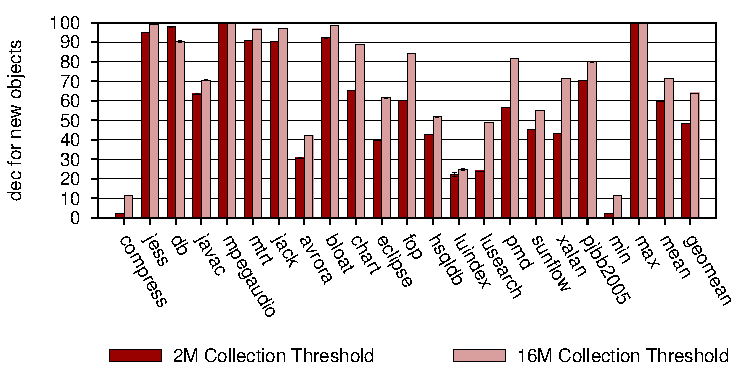
\includegraphics[width=\columnwidth]{figs/decnew}}
  \caption{New objects are responsible for the majority of reference
    counting operations.  We show here the fraction of (a) increments
    and (b) decrements that are due to objects allocated within the
    most recent 2\,MB and 16\,MB of objects allocated.}
  \label{fig:incdecnew}
\end{figure}

Figure~\ref{fig:incdecnew} is an example of a figure with subfloats
and an example of a reasonable caption.  Notice how the caption is
somewhat self-contained.  The reader could glance at this figure and
understand something of it without being required to dig into the
text. The graphs in Figure~\ref{fig:incdecnew} are too small --- only
just acceptable.

This is an example of using the \textsf{\textbackslash siunitx}
package: The job took \SI{321}{\micro\second}, with an average current
of \SI{3.24}{\ampere}, totalling \SI{1.13}{\milli\watt}.  These macros
ensure correct typsetting --- note the small space between number and
units and the non-italicized mu for the \si{\micro\second}.  The
package provides very powerfull options for formatting tables (not yet
used in the example given in this template!).  Check out the package
documentation.

\begin{table*}
  \newcommand{\timemetric}{$\Delta\mathsf{t}$}
  \newcommand{\instmetric}{$\Delta\mathsf{i}$}
  \newcommand{\imissmetric}{$\Delta\mathsf{i_{miss}}$}
  \newcommand{\cpimetric}{$\mathsmaller{\Delta\mathsf{t}/\Delta\mathsf{i}}$\xspace}
  \centering
   {  \relsize{-1}   % use relsize to scale the entire table uniformly.
  \input table/bigexample.tex
  }
  \caption{Overheads (\%) in time, instructions, and i-cache misses for the
    primitive barriers on the i7.  The the first six column groups summarize
    the performance for each barrier, showing percentage increase in
    execution time (\timemetric), retired instructions (\instmetric), and
    instruction cache misses (\imissmetric) compared to the base case where
    no barriers are used.  The right-most two column groups give results for
    the compound barriers.  The figures in grey beneath the corresponding
    arithmetic mean report 95\% confidence intervals.}
    \label{tab:big}
\end{table*}

Table~\ref{tab:big} is a pretty good example of a large table.  It's
probably the largest table we've ever published in a regular
conference paper.  Don't do it lightly.  A table like this should be
generated with a script or at least with the assistance of an emacs
macro.  There is a massive amount of information in this table, and
without very careful typesetting, it would be a disaster and
unreadable.
\\

\noindent
Notice:
\begin{enumerate}
\item that the font is sans serif,
\item that there are no vertical lines,
\item that differences in whitespace between the columns and breaks in
  the horizontal lines serve to group the data into clusters,
\item how the secondary (but nonetheless important) data about
  confidence intervals is typset in a very small font in grey,
\item how benchmark suites are separately aggregated and expressed in
  bold,
\item how both means and geomeans are provided, and
\item how mins and maxs across all the benchmarks are at the bottom.
\end{enumerate}

%%% Local Variables:
%%% mode: latex
%%% TeX-master: "paper"
%%% End:
